\SECTION{Design and Implementation}\label{sec:design_imple}
In this section, we present the design and implementation of Linux-RTXG,
which provides a framework of coordinated CPU and GPU resource
management with LKMs.
We describe our approach to GPU scheduling and its integration to CPU
scheduling.
Due to a space constraint, the detail of LKM-based CPU scheduling is
referred to the RESCH project~\cite{kato2009loadable, asberg2012exsched}.

\SUBSECTION{Linux-RTXG}
\begin{figure}[t]
\begin{center}
\ifthesis
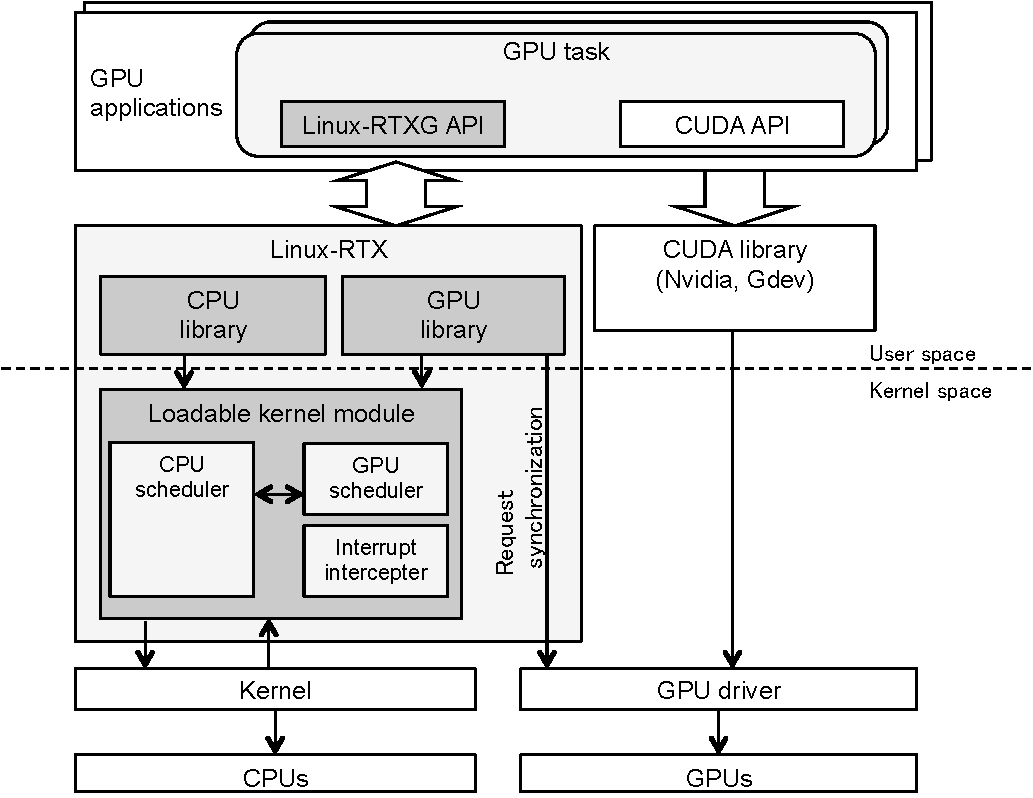
\includegraphics[width=0.8\textwidth]{img/overview.pdf}
\else
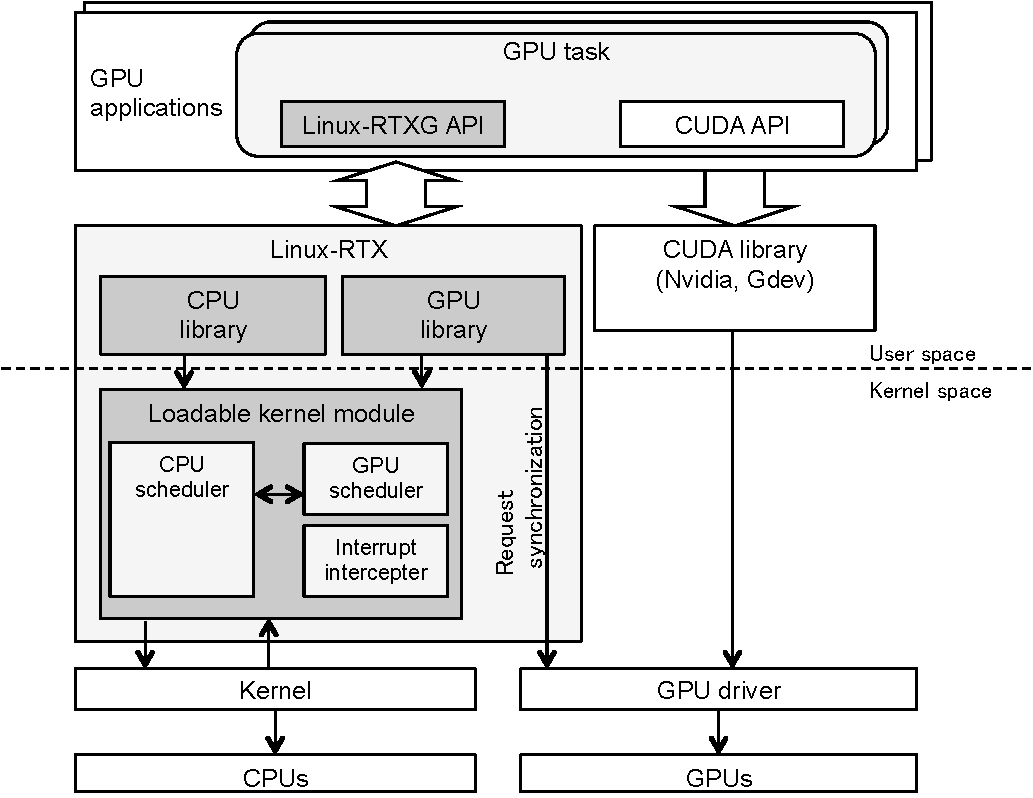
\includegraphics[width=0.35\textwidth]{img/overview.pdf}
\fi
\caption{Architectural overview of Linux-RTXG.}
\label{fig:overview}
\end{center}
\end{figure}

Figure~\ref{fig:overview} shows an architectural overview of
Linux-RTXG.
The system architecture of Linux-RTXG falls into two parts.
First, the Linux-RTXG core contains a CPU scheduler and a GPU scheduler
with a resource reservation mechanism.
The implementation of the Linux-RTXG core is provided in the kernel
space by an LKM.
Thus, it can use exported Linux kernel functions, such as $schedule()$,
$mod\_timer()$, $wake\_up\_process()$, and $set\_cpus\_allowed\_ptr()$.
These functions can be called from the user space interface using the
input/output control (ioctl) system call, which is a standard system
call for device drivers.
Secondly, the Linux-RTXG library contains an independent synchronization
method for coordinated CPU and GPU resource management.
The independent synchronization method can be used on top of a
proprietary driver~\cite{nvidia:cuda_zone} as well as an open-source
driver~\cite{nouveau}.
Note that this method is required to manage interrupts for GPU
scheduling without any code modification to the OS kernel and device
drivers.

\SUBSECTION{GPU Scheduling}
\begin{table*}[!t]
\begin{center}
\caption{A basic set of APIs for Linux-RTXG.}
\label{tab:rtx-api}
\ifthesis
\begin{tabular}{|l|p{25em}|} \hline
\else
\begin{tabular}{|l|p{50em}|} \hline
\fi
rtx\_gpu\_open() & Registers itself to Linux-RTXG and creates scheduling entity. It must be called first. \\ \hline
rtx\_gpu\_device\_advice() & Obtains recommendations for which GPU devices to use. \\ \hline
rtx\_gpu\_launch() & Controls GPU kernel launch timing, (i.e., a scheduling entry point). It must be called before the CUDA launch API. \\ \hline
rtx\_gpu\_sync() & Waits for the completion of GPU kernel execution by sleeping with TASK UNINTERRUPTIBLE status. \\ \hline
rtx\_gpu\_notify() & Sends NOTIFY/FENCE command to GPU. The FENCE/NOTIFY are selected by flag that is set by argument.\\ \hline
rtx\_gpu\_close() & Releases scheduling entity.\\ \hline
\end{tabular}
\end{center}
\end{table*}

Linux-RTXG is based on the interrupt-driven method for GPU
synchronization but is also partly based on the API-driven method.
The scheduler is invoked only when computation requests are submitted.
The basic APIs supported by Linux-RTXG are listed in Table~\ref{tab:rtx-api}.
Note that some APIs have arguments whereas others do not.
Linux-RTXG does not modify the existing CUDA API to cope with
proprietary software, being independent of GPU runtimes. 
However, CUDA application programs must add the Linux-RTXG APIs to use
the functionality of Linux-RTXG.

The sample code including the Linux-RTXG APIs is shown in
Figure~\ref{fig:sample}.
GPU tasks are provided with function calls to Linux-RTXG at strategic
points.

\begin{figure}[!t]
\begin{center}
\begin{tabular}{l}
\hline\hline
{\scriptsize \verb|void gpu_task(){        |}\\
{\scriptsize \verb| /* variable initialization  */        |}\\
{\scriptsize \verb| /* calling RESCH API */        |}\\
{\scriptsize \verb|  dev_id = rtx_gpu_device_advice(dev_id); |}\\
{\scriptsize \verb|  cuDeviceGet(&dev, dev\_id);           |}\\
{\scriptsize \verb|  cuCtxCreate(&ctx, SYNC_FLAG, dev);    |}\\
{\scriptsize \verb|  rtx_gpu_open(&handle, vdev_id);     |}\\
{\scriptsize \verb| /* Module load and set kernel function */ |}\\
{\scriptsize \verb| /* Device memory allocation        */ |}\\
{\scriptsize \verb| /* Memory copy to device from host */ |}\\
{\scriptsize \verb|  rtx_gpu_launch(&handle); |}\\
{\scriptsize \verb|  cuLaunchGrid(function, grid_x, grid_y); |}\\
{\scriptsize \verb|  rtx_gpu_notify(&handle); |}\\
{\scriptsize \verb|  rtx_gpu_sync(&handle);   |}\\
{\scriptsize \verb|  /* Memory copy to host from device */  |}\\
{\scriptsize \verb|  /* Release allocated memory */  |}\\
{\scriptsize \verb|}|}\\
\hline\hline
\end{tabular}
\caption{Sample code with the Linux-RTXG APIs.}
\label{fig:sample}
\end{center}
\end{figure}

\begin{figure}[!t]
\begin{center}
 \ifthesis
 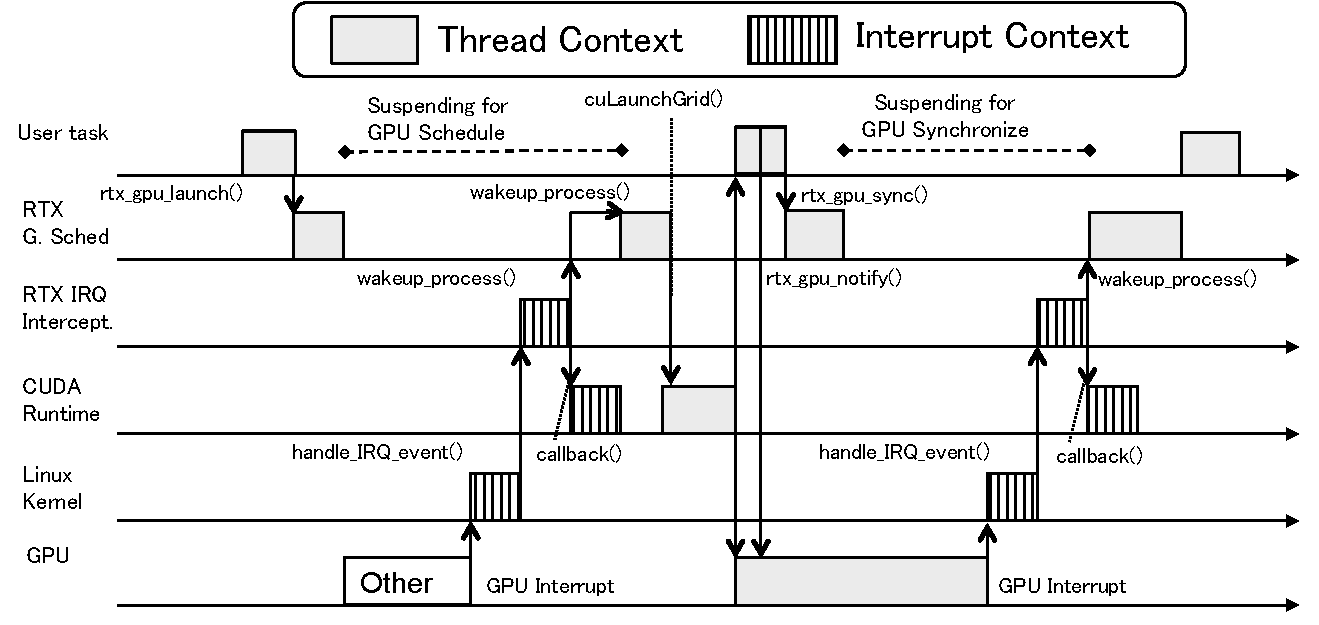
\includegraphics[width=\textwidth]{img/gsched_controlflow.pdf}
 \else
 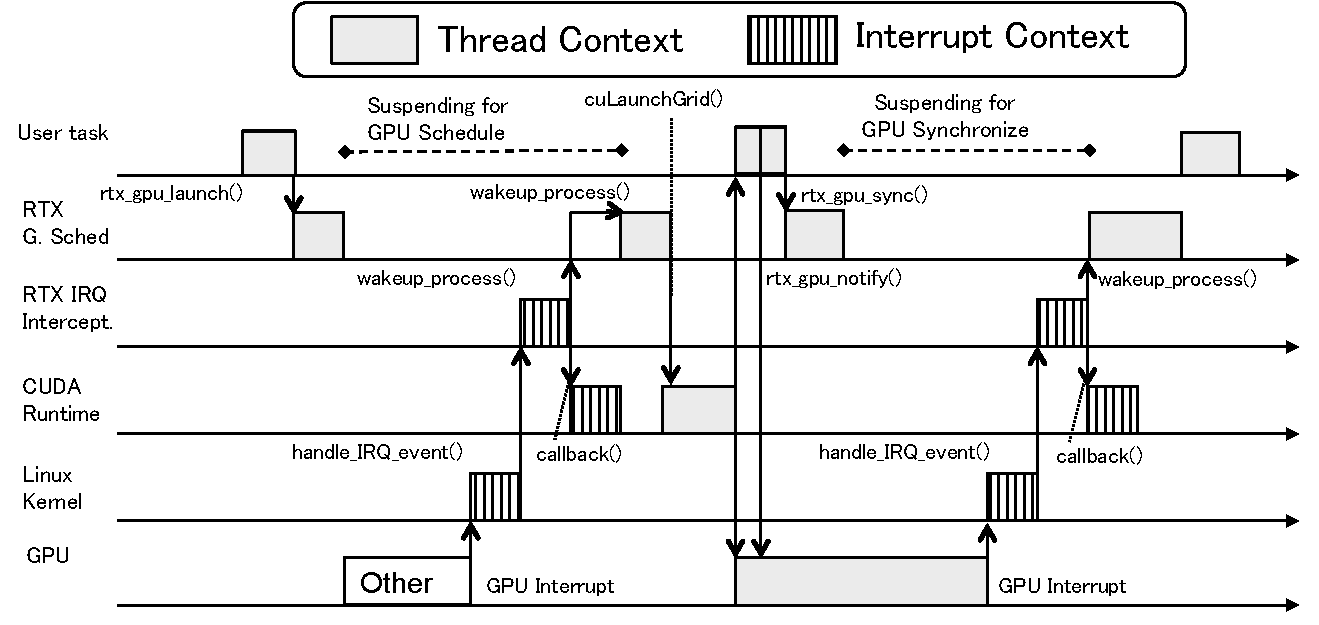
\includegraphics[width=0.5\textwidth]{img/gsched_controlflow.pdf}
 \fi
 \caption{Execution flow of the GPU task.}
 \label{fig:controlflow}
\end{center}
\end{figure}

The execution flow of the GPU task managed by the Linux-RTXG APIs is
described in Figure~\ref{fig:controlflow}.
Note that this example is restricted to a single GPU kernel.
The GPU task can control the timing of GPU kernel invocation by calling
$rtx\_gpu\_launch()$.
After this function call, the task is suspended until it receives an
interrupt so that other GPU kernels can be launched.
When some GPU kernel is completed, an interrupt is raised by the GPU and
the corresponding interrupt handler is executed by the Linux kernel.
The interrupt interceptor awakens some suspending task according to the
priority.
The awakened task proceeds to launch the GPU kernel using the CUDA API,
such as $cuLaunchGrid()$.
After the GPU kernel is launched, the task is going to register NOTIFY
to set up an interrupt, and is again put to the sleep mode until it
receives the interrupt.
Dispatching of the subsequent task is performed by the GPU scheduler,
which is called upon the interrupt from the GPU.
Linux-RTXG manages the order of task execution according to this flow.

We now present a hierarchal scheduling mechanism that uses the concept
of virtual GPUs to combine specified GPU tasks by a group.
The virtual GPUs are realized by a resource reservation mechanism, while
GPU scheduling uses a priority mechanism.
Specifically, each GPU kernel invocation is associated with a scheduling
entity, and Linux-RTXG allocates the scheduling entities to virtual GPUs. 
The virtual GPUs can belong to any physical GPUs.
In Linux-RTXG, computing resources are distributed to virtual GPUs.

Figure~\ref{fig:scheduling} shows the pseudo-code of the Linux-RTXG
scheduler.
This code works under the assumption that $on\_arrival$ is called when
some GPU task requests to launch the GPU kernel.
In $on\_arrival$, the GPU task checks whether the given execution
permission is held by the allocated virtual GPU and is also held by the
allocated scheduling entity.
If the virtual GPU to which the GPU task belongs does not own the
execution permission, the GPU task is enqueued to $wait\_queue$ and is
suspended.
Else, the GPU task can launch the GPU kernel.
After a while, $on\_completion$ is called by the scheduler thread when
the launched GPU kernel is completed, and we can select the next set of
a virtual GPU and a GPU task. 
At the end of $on\_completion$, the selected GPU task is waken up.

\begin{figure}[!t]
\begin{center}
\begin{tabular}{l}
\hline
{\scriptsize \verb| se: The scheduling entity |}\\
{\scriptsize \verb| se->vgpu: The group that belongs to se|}\\
{\scriptsize \verb| se->task: The task that is associated with se |}\\
{\scriptsize \verb| vgpu->parent: The physical GPU identification|}\\
\hline
{\scriptsize \verb|void on_arrival(se) {|}\\
{\scriptsize \verb| check_permit_vgpu(se->vgpu)    |}\\
{\scriptsize \verb| while(!check_permit_se(se)){|}\\
{\scriptsize \verb|   enqueue(se->vgpu,se); |}\\
{\scriptsize \verb|   sleep_task(se->task); |}\\
{\scriptsize \verb|}}|}\\
{\scriptsize \verb|void on_completion(se) {|}\\
{\scriptsize \verb| reset_the_permit(se->vgpu, se)|}\\
{\scriptsize \verb| n_vgpu = pick_up_the_next_vgpu(se->vgpu->parent) |}\\
{\scriptsize \verb| se = pick_up_the_next_se(n_vgpu)|}\\
{\scriptsize \verb| if(se) {|}\\
{\scriptsize \verb|   dequeue(se->vgpu,se);|}\\
{\scriptsize \verb|   wakeup_task(se->task);|}\\
{\scriptsize \verb| }|}\\
{\scriptsize \verb| set_the_permit(se->vgpu, se)|}\\
{\scriptsize \verb|}|}\\
\hline
\end{tabular}
\caption{High-level pseudo-code of the Linux-RTXG scheduler.}
\label{fig:scheduling}
\end{center}
\end{figure}

\SUBSECTION{GPU Synchronization}
Here, we describe the independent synchronization mechanism and the interrupt intercept.
The independent synchronization mechanism invokes NOTIFY and FENCE without using a GPU runtime API.
The interrupt intercept realizes interrupt-driven wakeup of the scheduler without kernel modification.
Linux-RTXG uses the independent synchronization mechanisms as much as possible
because we do not want to use black--box resource management.

\textbf{Independent synchronization mechanism from runtime:}
We present an independent synchronization mechanism for NOTIFY and FENCE.
The mechanism invokes an interrupt for NOTIFY, and writes the fence value with the GPU microcontrollers for FENCE.
NVIDIA's proprietary software uses the ioctl interface to communicate between the kernel-space and the user-space.
These ioctl interfaces provide driver functions, such as device memory allocation, obtaining GPU information and memory mapping.
Gdev builds infrastructure that can execute on NVIDIA's driver using these ioctl interfaces.
The proposed method uses an ioctl interface similar to Gdev's method for sending commands.
Specifically, the proposed method is divided into two parts, Initialize and Notify.
Initialize processess generate a dedicated GPU context.
This processess include creating virtual address space, allocating an indirect buffer object for sending a command, and creating a context object is required to prepare the FIFO engine and includes, allocating a kernel memory object and mapping the FIFO engine register to host memory space using memory-mapped I/O.
The FIFO engine is a GPU microcontroller that receives commands.
The Notify processes send commands to a compute engine or a copy engine by $iowrite$ function to the mapped FIFO engine's register.
The compute engine and the copy engine do function that switching a GPU context for computing or data copy.
This independent synchronization mechanism uses reverse engineering.
Therefore, this method depends on the GPU device architecture and the proprietary software interfaces.

\textbf{Interrupt interception:}
Interrupts are handled by the ISR registered to the kernel by the device driver.
In addition, a scheduler is required to receive the interrupt and to identify the interrupt by reading the GPU status register.
The GPU status register must be read before the original ISR resets the GPU status register.

The Linux kernel has structures that hold interrupt parameters called $irq\_desc$ for each interrupt number.
These structures have structures called $irq\_action$, including the ISR callback pointer.
An $irq\_desc$ is allocated to global kernel memory space, and is freely accessible from kernel space.
Linux loadable kernel modules can obtain an $irq\_desc$ and an ISR callback pointer.
We obtain the GPU device driver's ISR callback pointer, and then we register an interrupt interception ISR to the kernel.
Thus, we obtain an interrupt interception from the interrupt interception ISR and retain the callback pointer.
In addition, I/O registers are mapped to kernel memory space by the device driver from the PCIe base address registers (BAR)~\cite{fujii:icpads2013,kato2013zero}.
Therefore, Linux-RTXG remaps the BAR0 to our allocated space using $ioremap()$ when the ISR initialized.
The interrupt interception identifies an interrupt by reading this mapped-space.

\SUBSECTION{Scheduler Integration}
The native Linux scheduler has various real-time scheduling policies, such as $SCHED\_DEADLINE$, $SCHED\_FIFO$ and $SCHED\_RR$.
$SCHED\_DEADLINE$ is an implementation of a constant bandwidth server and a global earliest deadline first.
$SCHED\_DEADLINE$ is included in the Linux 3.14.0 kernel.
However, synchronization does not work well with the SCHED\_DEADLINE scheduling policy for GPU tasks.
Here there are two problems.
The first is the implementation of $sched\_yield$---.$sched\_yield()$ uses $yield()$ in kernel space---.
The second is the implementation of waking from a sleeping state.

The first problem occurs by releasing the CPU using $sched\_yield()$ while waiting for I/O in polling.
Polling (spin) is the exclusive CPU; therefore, a task may once better to release the CPU can obtain good results.
However, $sched\_yield$ will set the polling task's remaining execution time to 0 by treating it as a parameter of $SCHED\_DEADLINE$.
Thus, the task cannot execute until the runtime is replenished in the next period.
Therefore, the task cannot call $sched\_yield()$ between polling.
$sched yield()$ is frequently used by device drivers and libraries, as well as GPU environment, and such software is affected by this problem.
Depending on the setting, even NVIDIA's CUDA can be affected by this problem.
We address this problem by limiting the GPU synchronization method to NOTIFY in the $SCHED\_DEADLINE$ policies.

The second problem is subjected to a check equation~\ref{eq} when restoring a task from the sleep state.
If equation~\ref{eq} holds, the runtime is replenished and absolute deadline is set to the next cycle deadline.

{\scriptsize
\begin{equation}
\frac{Absolute\_Deadline - Current\_Time}{Remaining\_Runtime} > \frac{Relative\_Deadline}{Period} \label{eq}
\end{equation}
}

We implement this check by subtracting GPU execution time from $Remaining Runtime$ when a task is restored by GPU kernel execution, with the exception of a task that is restored by period.
